\section{Visualización y asignación del Issue}

Para revisar los detalles del nuevo Issue se utilizó el siguiente comando:

\begin{lstlisting}
gh issue view 8 --repo martinezmoralesdiego2020-droid/repositorio
\end{lstlisting}

Al visualizar la incidencia se observó que todavía no tenía un responsable asignado.

\begin{figure}[H]
\centering
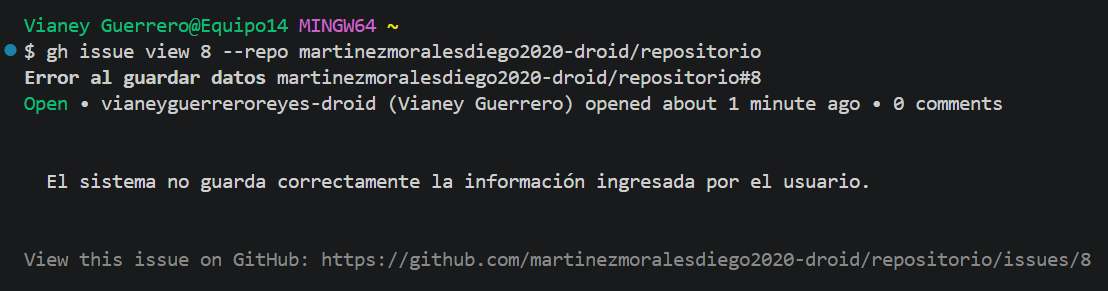
\includegraphics[width=0.9\textwidth]{M8.png}
\caption{Visualización del Issue \#8 antes de asignar un responsable.}
\end{figure}

Posteriormente se asignó la incidencia al integrante Diego Martínez mediante el comando:

\begin{lstlisting}
gh issue edit 8 --add-assignee martinezmoralesdiego2020-droid --repo martinezmoralesdiego2020-droid/repositorio
\end{lstlisting}

Con ello se estableció formalmente al responsable encargado de atender el problema reportado y se volvió a visualizar el Issue para verificar que la asignación hubiera sido realizada correctamente.


\begin{figure}[H]
\centering
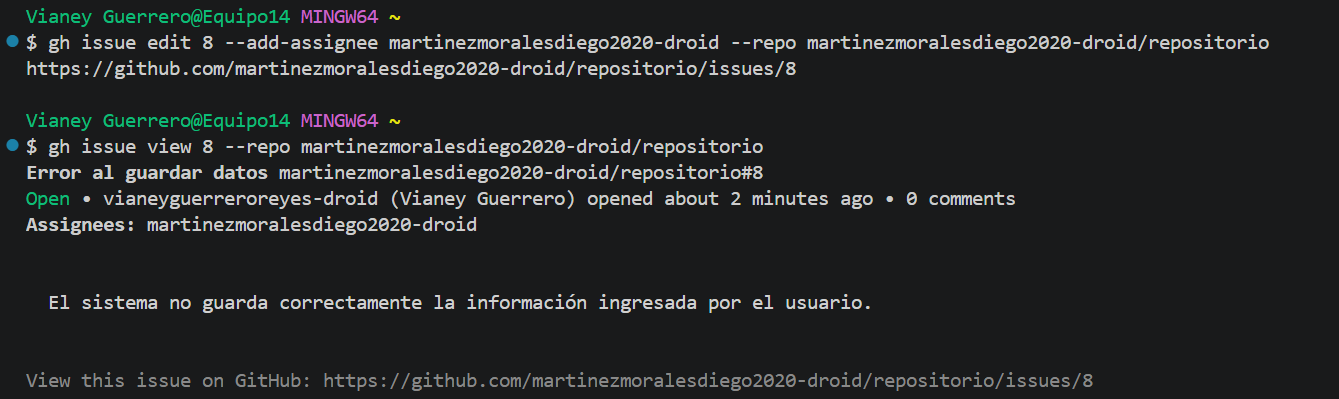
\includegraphics[width=0.9\textwidth]{M9.png}
\caption{Asignación del Issue \#8 al integrante Diego Martínez.}
\end{figure}
